\documentclass[11pt]{beamer}
\usetheme{Dresden}
\usecolortheme{beaver}
\usepackage[utf8]{inputenc}
\usepackage{amsmath}
\usepackage{amsfonts}
\usepackage{amssymb}
\usepackage{graphicx}
\usepackage{verbatim}
\usepackage{listings}
\usepackage{xcolor}

\let\OldTexttt\texttt
\renewcommand{\texttt}[1]{\OldTexttt{\color{teal}{#1}}}

\definecolor{mGreen}{rgb}{0,0.6,0}
\definecolor{mGray}{rgb}{0.5,0.5,0.5}
\definecolor{mPurple}{rgb}{0.58,0,0.05}
\definecolor{mGreen2}{rgb}{0.05,0.65,0.05}
\definecolor{mGray2}{rgb}{0.55,0.55,0.55}
\definecolor{mPurple2}{rgb}{0.63,0.05,0.05}
\definecolor{backgroundColour}{rgb}{0.95,0.95,0.92}
\definecolor{backgroundColour2}{rgb}{0.95,0.92,0.95}

\lstdefinestyle{C}{
    backgroundcolor=\color{backgroundColour},   
    commentstyle=\color{mGreen},
    keywordstyle=\color{blue},
    numberstyle=\tiny\color{mGray},
    stringstyle=\color{mPurple},    
    basicstyle=\footnotesize,
    breakatwhitespace=false,         
    breaklines=true,                 
    captionpos=b,                    
    keepspaces=true,                 
    numbers=left,                    
    numbersep=5pt,                  
    showspaces=false,                
    showstringspaces=false,
    showtabs=false,                  
    tabsize=2,
    language=C
}

\lstdefinestyle{Python}{
    backgroundcolor=\color{backgroundColour2},   
    commentstyle=\color{mGreen2},
    keywordstyle=\color{blue},
    numberstyle=\tiny\color{mGray2},
    stringstyle=\color{mPurple2},
    basicstyle=\footnotesize,
    breakatwhitespace=false,         
    breaklines=true,                 
    captionpos=b,                    
    keepspaces=true,                 
    numbers=left,                    
    numbersep=5pt,                  
    showspaces=false,                
    showstringspaces=false,
    showtabs=false,                  
    tabsize=2,
    language=Python
}

\author{NCC Moore}
\title{Topic 4 - Arrays and Introductory Algorithms}
%\setbeamercovered{transparent} 
%\setbeamertemplate{navigation symbols}{} 
%\logo{} 
\institute{McMaster University} 
\date{Fall 2020} 
\subject{SFWRENG 2MP3 - Programming for Mechatronics} 
\stepcounter{section}
\begin{document}

\begin{frame}
\center
SFWRENG 2MP3 - Programming for Mechatronics
\titlepage
(Loosely) Adapted from Chapter 6 of C: How to Program 8th ed., Deitel \& Deitel
\end{frame}

\begin{frame}
\tableofcontents
\end{frame}

\section[Arrays]{Arrays: Like Tuples, But More Annoying} % include 6.6, 6.7
\begin{frame}{Arrays: The Simplest Data Structure}
\center
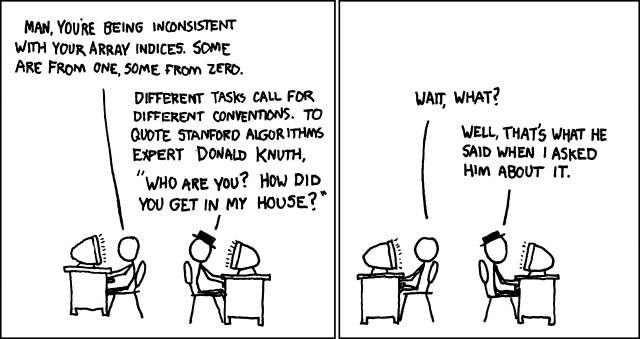
\includegraphics[scale=3]{donald_knuth.png} \\
The joke within the joke is that hat guy imagines he has a choice... \\ 
-- Your Professor -- 
\end{frame}

\begin{frame}{I see data \texttt{Array}ed before me...}
In Python, there are many data structures to choose from:
\begin{itemize}
\item Tuples
\item Lists
\item Dictionaries
\item Sets
\item Strings
\end{itemize}
In C, the only data structure supported natively is the \textbf{Array}.  If you need something more complex than an Array, you have to either find a library defining it or define it yourself. 
\end{frame}

\begin{frame}{So what is an \texttt{Array}?}
An array is a contiguous segment of memory, which may be accessed via linear indexing.
\begin{itemize}
\item All elements of an array have the same type.
\item Arrays use \textbf{zero-indexing}.
\item Arrays are \emph{static}
\begin{itemize}
\item The size of an array does not change during execution
\item This means that the size of the array \emph{must} be known at the time of declaration.  
\item There are ways of getting around this, but not without pointers (which we'll be talking about soon...)
\end{itemize}
\end{itemize}
\end{frame}

\begin{frame}[fragile=singleslide]{Syntax, my friends!}
An array is declared in the following manner:
\begin{lstlisting}[style=C]
int c[x];
\end{lstlisting}
\begin{itemize}
\item Note, that $x$ must be either an integer literal or an expression which evaluates to an integer. 
\begin{itemize}
\item This rule applies to array indexing as well as declaration.
\end{itemize} 
\item On declaration, an array is filled with \emph{junk data!}
\end{itemize}
Arrays may be indexed using the array index operator:
\begin{lstlisting}[style=C] 
c[7] = 5;
\end{lstlisting} 
\begin{itemize}
\item Binds at the same level as function calls (so very tightly)
\item As we'll see later, the index operator is syntactic sugar for some pointer operations.
\end{itemize}
\end{frame}

\begin{frame}[fragile=singleslide]{Pretty Printing Arrays}
\begin{lstlisting}[style=C] 
#include <stdio.h>
int main () {
	int c[(6+6)];
	float bar[] = {0.0, 0.1, 0.2, 0.3};
	printf("%d\n", c);
	printf("%p\n", c);
	printf("[");
	for (int i = 0; i < 12; i++) {
		if (i < 11) {
			printf("%d, ", c[i]);
		} else {
			printf("%d]\n", c[i]);
		}
	}
}
\end{lstlisting} 
\end{frame}

\begin{frame}{Pretty Printing Arrays (Visualization)}
\center
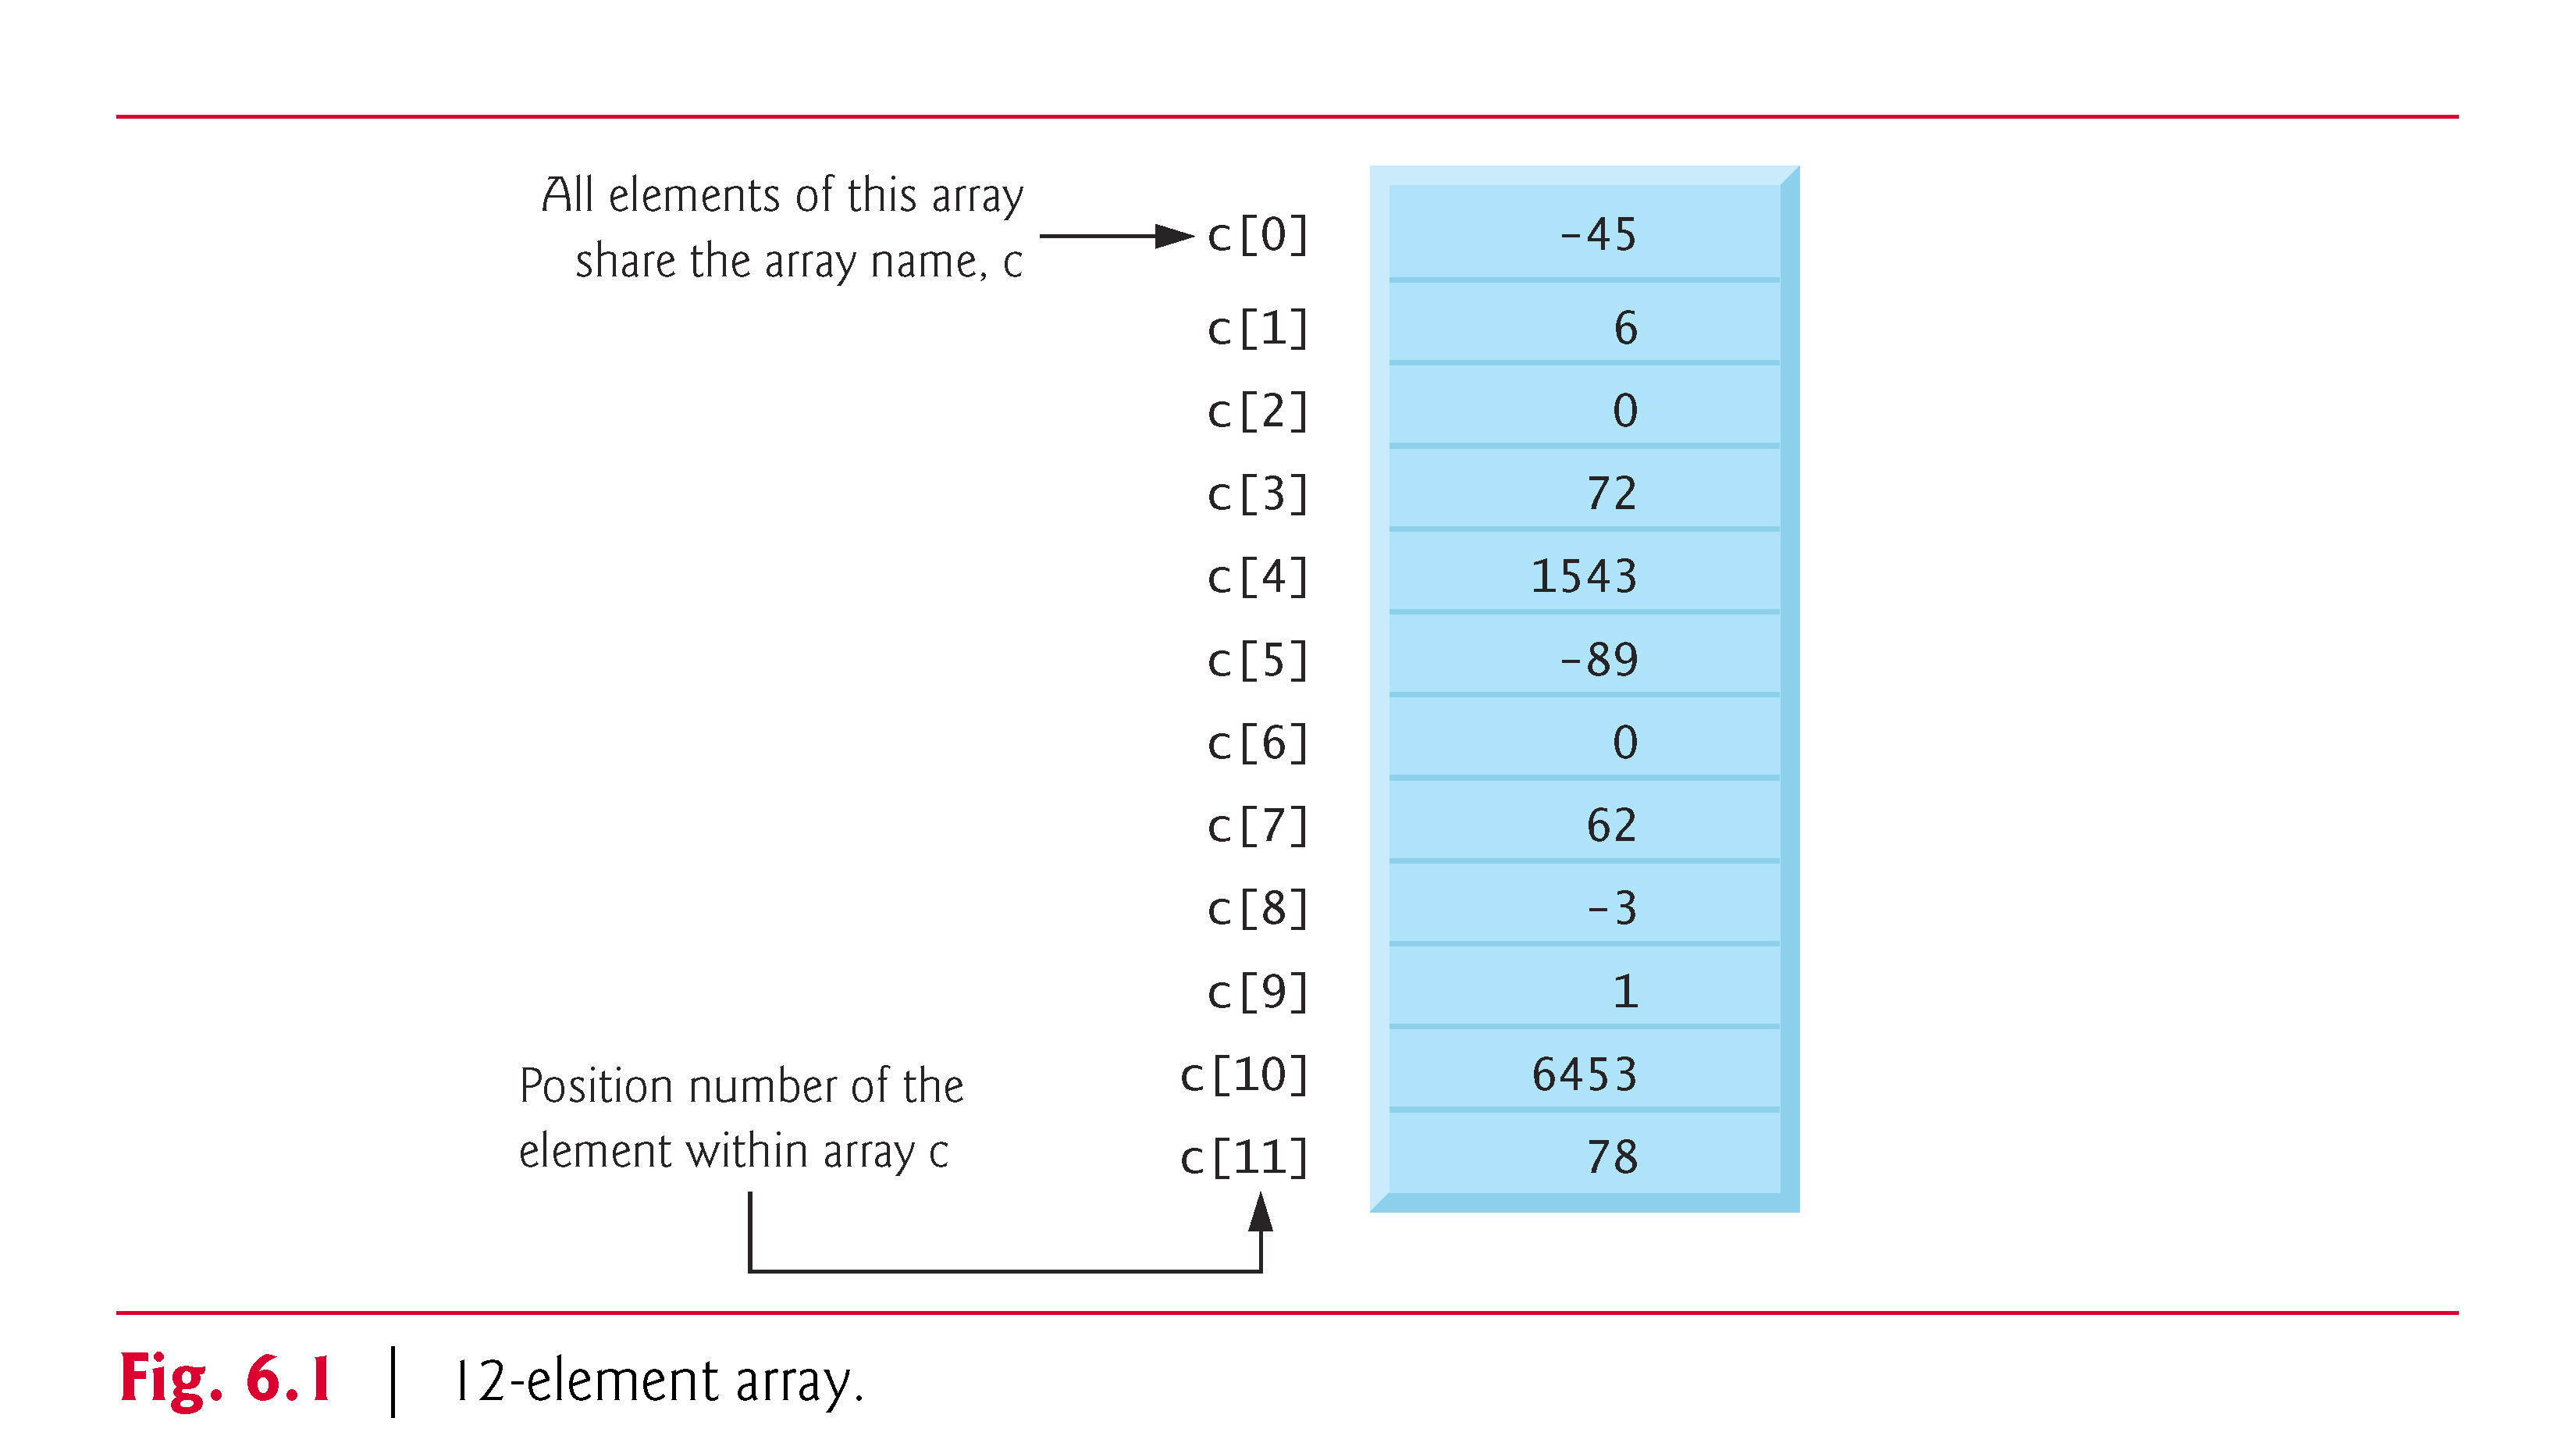
\includegraphics[scale=0.1]{array.png}
\end{frame}

\begin{frame}[fragile=singleslide]{Pretty Printing Arrays (output)}
Compiler Warnings:
\begin{verbatim}
In function ‘main’:
warning: format ‘%d’ expects argument of type ‘int’, 
  but argument 2 has type ‘int *’
  printf("%d\n", c);
          ~^     ~~~
          %ls
\end{verbatim}
Output:
\hrule
\begin{verbatim}
-1506989472
0x7ffca62d2a60
[1, 0, 56797197, 22077, 997394928, 32685, 0, 0, 
  56797120, 22077, 56796656, 22077]
\end{verbatim}
\end{frame}

\begin{frame}{Pretty Printing Arrays (Analysis)}
Just like with a lot of things in C, there are no free lunches! 
\begin{itemize}
\item You can't print a whole array just by passing the array's name to \texttt{printf} as the array identifier is really a \textbf{memory address}, or \textbf{pointer}.
\end{itemize}
Initialization!
\begin{itemize}
\item An uninitialized array is full of garbage data! 
\item To initialize an array, provide a comma separated series of type-correct literals or expressions, delimited with curly braces! 
\item If the initializer is smaller than the declared memory, C backfills with zeros!
\item If you initialize the array, you may omit specifying the size (the size of the initializing array will be used).
\end{itemize}
\end{frame}

\begin{frame}[fragile=singleslide]{Macro, Macro Man!}
It seems like kind of a pain to have to hard-code our array sizes... There has to be a better way! 
\begin{lstlisting}[style=C]
#define SIZE 256
\end{lstlisting}
\begin{itemize}
\item A \textbf{Macro} is preprocessor command which defines a character substitution that occurs prior to compilation.  
\item Think of it as an automatic find-and-replace operation.
\item We may use macros to replace all occurances of the string \texttt{SIZE} with the size we wish our array to be, enhancing modularity! 
\item Macros can actually be used for all kinds of things... which we'll talk about in a later lecture! 
\end{itemize}
\end{frame}

\begin{frame}[fragile=singleslide]{Arrays and Functions}
Consider the following function prototype:
\begin{lstlisting}[style=C]
int* myFun (const int input[]);
\end{lstlisting}
\begin{itemize}
\item \texttt{input} is declared as an array by the inclusion of \texttt{[]}
\begin{itemize}
\item \texttt{int*} is also valid.
\end{itemize}
\item \texttt{int*} tells us that this function returns an \textbf{integer pointer}
\begin{itemize}
\item Arrays in C are syntactic sugar for pointers.
\end{itemize}
\item the \texttt{const} term locks the pointer so that it can't be modified.  This essentially makes it ``read-only''
\begin{itemize}
\item This will prevent any of the array's elements from being modified, as well as the value of the pointer.  
\item If you want to be able to modify the array, just leave out the \texttt{const} keyword.
\item You can do this with any argument, not just arrays!
\end{itemize}
\end{itemize}
\end{frame}

\begin{frame}[fragile=singleslide]{texttt{sizeof}}
In Python, we have the \texttt{len()} function to quickly and easily tell us how large our data structures are.  
\begin{itemize}
\item The equivalent fuction in C is \texttt{sizeof()}, but as with most things in C, it's a bit more complicated.
\item \texttt{sizeof()} returns the size \emph{in bytes} that the provided argument was declared with.   
\item \texttt{sizeof()} may be used on variables of any type, not just arrays.
\item Accordingly, the \emph{declared} length of an array is equal to the size of the array (in bytes) divided by the size of any element of the array (in bytes):
\begin{lstlisting}[style=C]
int foo[] = {1,2,3,4,5,6}
length = sizeof(foo) / sizeof(foo[0]);
\end{lstlisting}
\end{itemize}
\end{frame}

\begin{frame}[fragile=singleslide]{Accessing Higher Dimensions}
Linear arrays are all well and good, but what if I need to represent a matrix? 
\begin{lstlisting}[style=C]
// Declaring a 2D array
int foo[][] = {{1, 2}, {3, 4}};
// Declaring a 3D array
int bar[5][5][5];
\end{lstlisting}
\begin{itemize}
\item Dimensionality is indicated by the number of square braces following the identifier.
\item These are correctly thought of as \emph{arrays of arrays}.
\item Providing $n-k$ indexes to an $n$ dimensional array will produce a $k$ dimensional array.
\end{itemize}
\end{frame}

\section[String]{Strings are Character Arrays!} 
\begin{frame}{Strings are Character Arrays!}
\center
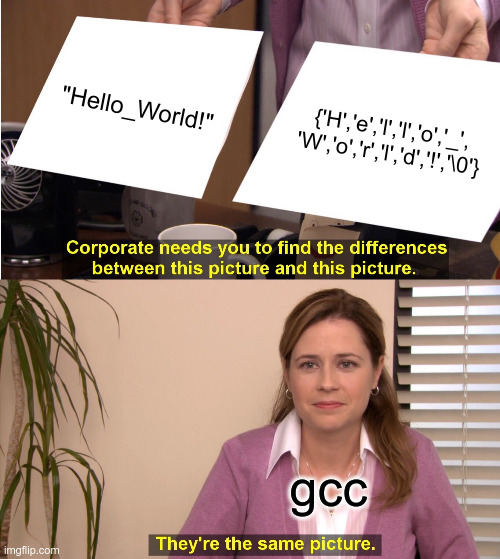
\includegraphics[scale=0.3]{charArrays.jpg}
\end{frame}

\begin{frame}[fragile=singleslide]{Character Arrays, not Character Sheets...}
As it turns out, C handles strings as \textbf{character arrays.} Consider the following declarations:
\begin{lstlisting}[style=C]
char foo[] = "bar";
\end{lstlisting}
\texttt{foo} will be written into memory as:
\begin{center}
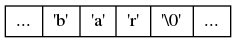
\includegraphics[scale=0.5]{graphs/string.png}
\end{center}
If we specify a size of ten,
\begin{lstlisting}[style=C]
char foo[10] = "bar"
\end{lstlisting}
 we get the following:
 \begin{center}
 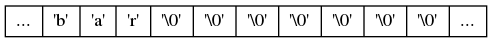
\includegraphics[scale=0.5]{graphs/string2.png}
 \end{center}

\end{frame}

\begin{frame}[fragile=singleslide]{String Things}
\begin{itemize}
\item \texttt{string} isn't even a keyword in C! 
\item Character arrays may be indexed, just like regular arrays.
\item String literals are always terminated by the \textbf{null character} implicitly!
\item All strings must be null terminated.
\item We can receive strings directly from \texttt{scanf} using the\texttt{\%s} format specifier.
\begin{lstlisting}[style=C]
scanf("%14s", foo);
\end{lstlisting}
\item By inserting a number, the format specifier may even be used to limit the number of characters that get copied into the character array.  
\item \texttt{foo} is actually a \textbf{pointer}, so we don't need the address-of operator \texttt{\&} in scanf. \texttt{foo} is already a memory address.
\end{itemize}
\end{frame}

\begin{frame}{Overflow Attacks!}
A common form of security vulnerablility in C and C++ programs is \textbf{array overflow}. 
\begin{itemize}
\item Arrays are replaced with pointer arithmetic by the compiler, with no bounds checking!  
\item If you tell C to write 100 characters into a 50 character array, it will happily do so! 
\item The extra 50 characters will be written into the memory that comes after the character array.
\item This can overwrite all kinds of useful things, like other variables.  If the character array is stored in the stack, function call informaton can also be vulnerable.  
\end{itemize}
The moral of the story is that you should always limit the things you write into an array to the size of the array MANUALLY! 
\end{frame}

\begin{frame}[fragile=singleslide]{Smash that Stack!}
\begin{lstlisting}[style = C]
#include <stdio.h>

int main() {
	char query[10];
	printf("Enter A Query : ");
	scanf("%s", query);
	printf("The query is %s\n", query);
}
\end{lstlisting}
\hrule
\begin{verbatim}
Enter A Query : jjjjjjjjjjjjjjjjjjjjjjjjjjjjjjj
The query is jjjjjjjjjjjjjjjjjjjjjjjjjjjjjjj
*** stack smashing detected ***: <unknown> terminated
	Aborted (core dumped)
\end{verbatim}
\end{frame}

\section[Bubble]{Bubblesort!}
\begin{frame}{Sort Yourself Out!}
\center
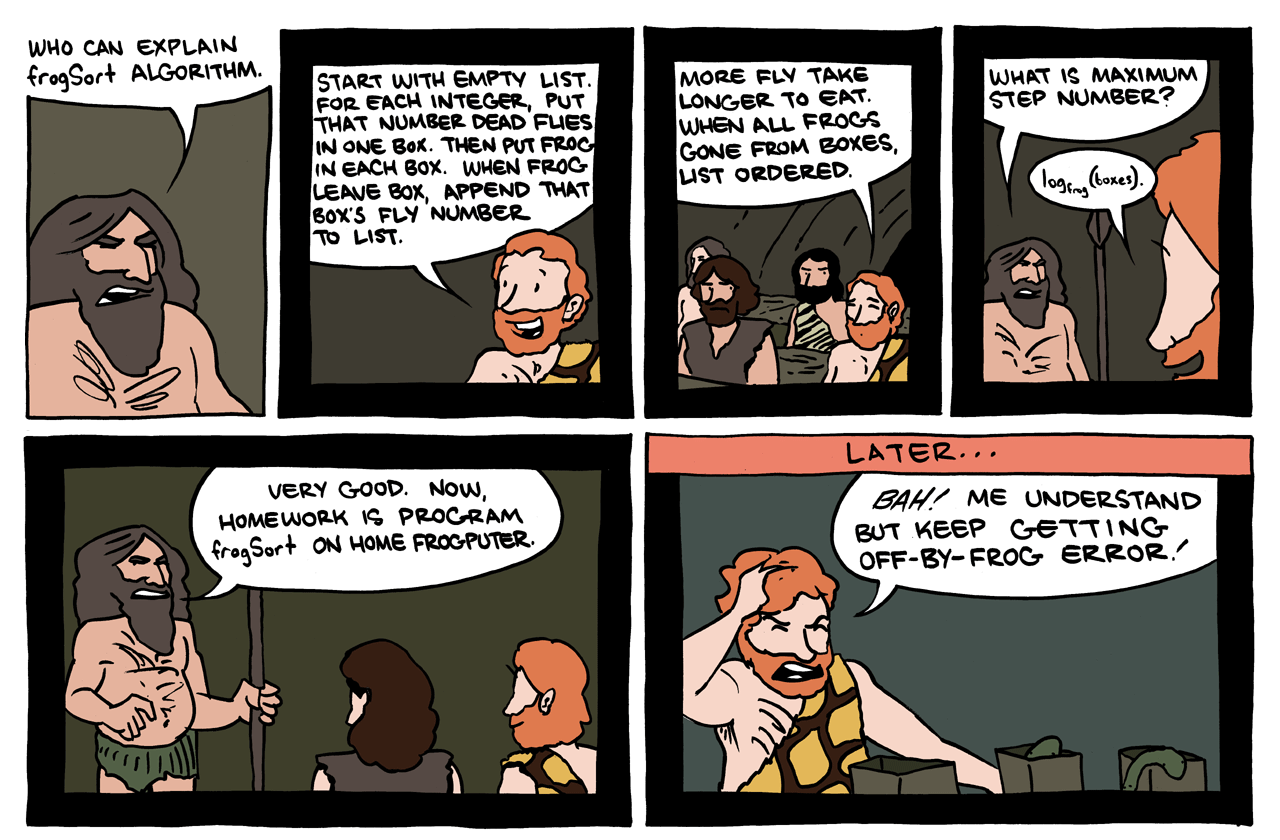
\includegraphics[scale=0.2]{frogsort.png}
\end{frame}

\begin{frame}{The Importance of Sorting Algorithms}
Sorting algorithms are one of the oldest areas of algorithm research
\begin{itemize}
\item The first formal analyses began in the 1950s
\item Many are necessary because there is no ``best algorithm''
\item Different sorts perform better in different conditions.
\begin{itemize}
\item How sorted the list is to begin with
\item Whether you optimize for runtime, memory, or call stack usage
\end{itemize}
\end{itemize}
Despite the venerable status of sorting algorithm research, advances are still being made!
\begin{itemize}
\item \textbf{Timsort} (2002) - Python's standard sorting algorithm: uses ordered subsequences to improve performance
\item \textbf{librarysort} (2006) - Allocates extra memory to ``gaps'', which allow the insertion of entries without reorganizaton of the entire array.
\end{itemize}
\end{frame}

\begin{frame}{So how is a sorting algorithm defined?}
A \textbf{Sorting Algorithm} is used to rearrange a given array or list elements according to a comparison operator on the elements. The comparison operator is used to decide the new order of element in the respective data structure. 
\begin{itemize}
\item Input: An array of values of arbitrary size 
\item Output: An array of values of the same size, in which the values are in ascending order.  
\end{itemize}
\center
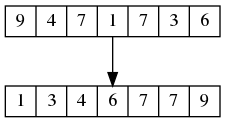
\includegraphics[scale=0.5]{graphs/sort.png}
\end{frame}

\begin{frame}{Bubblesort!}
Bubblesort's basic operation is to examine two numbers, and swap them if they are in the wrong order.  
\begin{itemize}
\item Starting at the beginning of the array, bubblesort examines each pair of consecutive elements in the order they occur.
\item After one pass through the array, the item at the end of the array is guaranteed to be in the right place.  
\begin{itemize}
\item The next pass can safely ignore it.
\end{itemize}
\item Bubblesort will make $n-1$ passes, given an array of size $n$.  
\item By the end of the $(n-1)^{th}$ pass, the whole array is guaranteed to be sorted! 
\end{itemize}
\end{frame}
% bubblesort

\begin{frame}{Visualizing Bubblesort}
\center
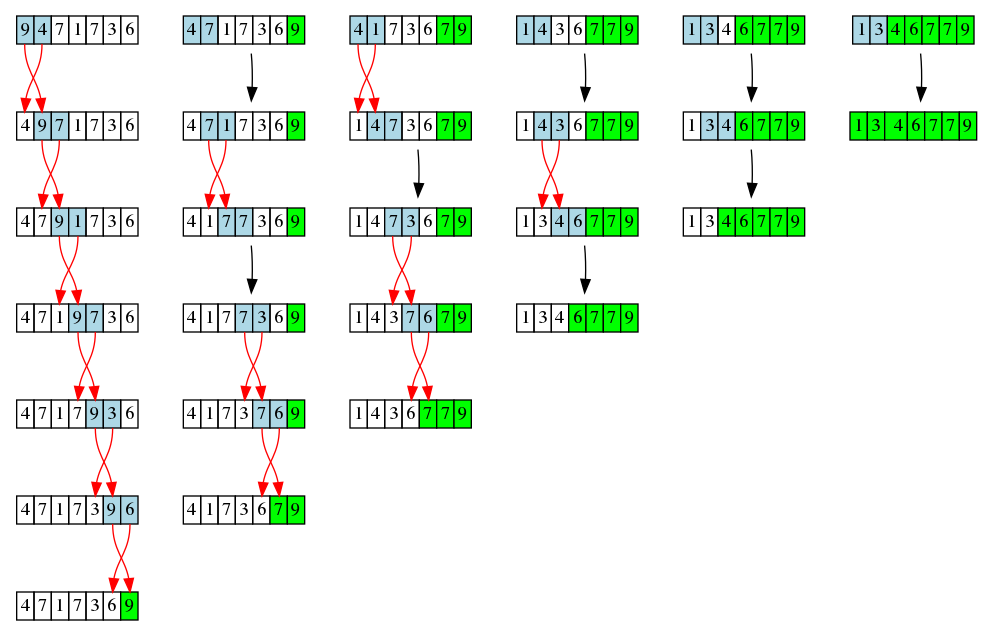
\includegraphics[scale=0.25]{graphs/bubblesort.png}
\end{frame}

\begin{frame}{Analyzing Our Example}
\begin{itemize}
\item The number of swap operations we required in the previous example was 13.   
\item The total number of examinations was 21, for an array of size 7.
\begin{itemize}
\item For each additional element in the array, we add $n-1$ to the total number of examinations.
\item This means that the total number of operations is proportional to the \textbf{square} of the size of the array.
\item We say the complexity of this algorithm is $O(n^2)$
\end{itemize}
\item Bubblesort can't tell the number of swaps that are needed before it makes a pass.
\begin{itemize}
\item The same number of examinations will occur, regardless of the orderedness of the array.
\item Therefore, we say that the \textbf{best case runtime} is equal to the \textbf{worst case runtime}.
\end{itemize}
\end{itemize}
\end{frame}

\section[Big O]{Big O Notation}
\begin{frame}{Big O Notation}
The mathematical analysis of the performance characteristics of algorithms is an entire subdiscipline of research within software engineering and computer science.
\begin{itemize}
\item It's quite difficult to measure software runtime
\begin{itemize}
\item Different computers will have different runtimes
\item The same computer with different operating systems will have different runtimes
\item Something like a comprehensive survey of all computer systems is impractical...
\end{itemize}
\item The algorithms community has made some decisions about what is important and what is unimportant with respect to measuring algorithmic efficiency.
\item Generally speaking, the time it takes a system to execute an instruction is unimportant, compared to \emph{how quickly the runtime grows, with respect to the size of the input}.
\end{itemize}
\end{frame}

\begin{frame}{Relating Input to Output}
So what is meant by ``the size of the input''?
\begin{itemize}
\item Generally, this refers to the size of the data structure the algorithm is applied to.
\item In the case of bubblesort, the size of the input is the number of items that are in the array to be sorted.  
\end{itemize}
In general, the relation of the input to the runtime can be expressed by a mathematical expression. Consider the following equation:
$$ R = an^2 + bn + c $$
\begin{itemize}
\item For the purposes of classifying algorithms, we are only concerned with the ``largest'' term in the expression.  
\end{itemize}
\begin{flushright}
\emph{continued on next slide...}
\end{flushright}
\end{frame}

\begin{frame}{Relating Input to Output (cont.)}
\begin{itemize}
\item This is because, for large values of n, the runtime will be mostly (even overwhelmingly) determined by the term with the highest power of n.  
\item We also don't care about the constants $a$, $b$, and $c$.
\begin{itemize}
\item This is where the individual differences between computer systems will show up
\item The constants are also effected by the specifics of algorithm implementation.
\item Reducing these constant terms is an active and important area of research.
\end{itemize}
\item In terms of bubblesort...
\begin{itemize}
\item the power of $n$ is how many times you have to examine/swap
\item the constant term is how long it takes you to examine/swap
\end{itemize} 
\end{itemize}
\end{frame}

\begin{frame}{Back to Big O}
An algorithm's runtime equation is \emph{abbreviated} into Big O notation:
$$ an^2 + bn + c \longrightarrow O(n^2) $$
\begin{itemize}
\item We often refer to this as the \textbf{complexity} of the algorithm.  
\item The complexity can be different in the best, worst, and average cases, and this can matter.
\item We can often tell what the complexity is by looking at the algorithm:
\begin{itemize}
\item Looping algorithms are $O(n^k)$, where $k$ is the number of nested loops 
\item Recursive algorithms which reduce the size of the input by half every step are generally $O(log_2(n))$
\end{itemize}
\end{itemize}
\end{frame}

\begin{frame}{Visualizing Different Runtime Complexities}
\center
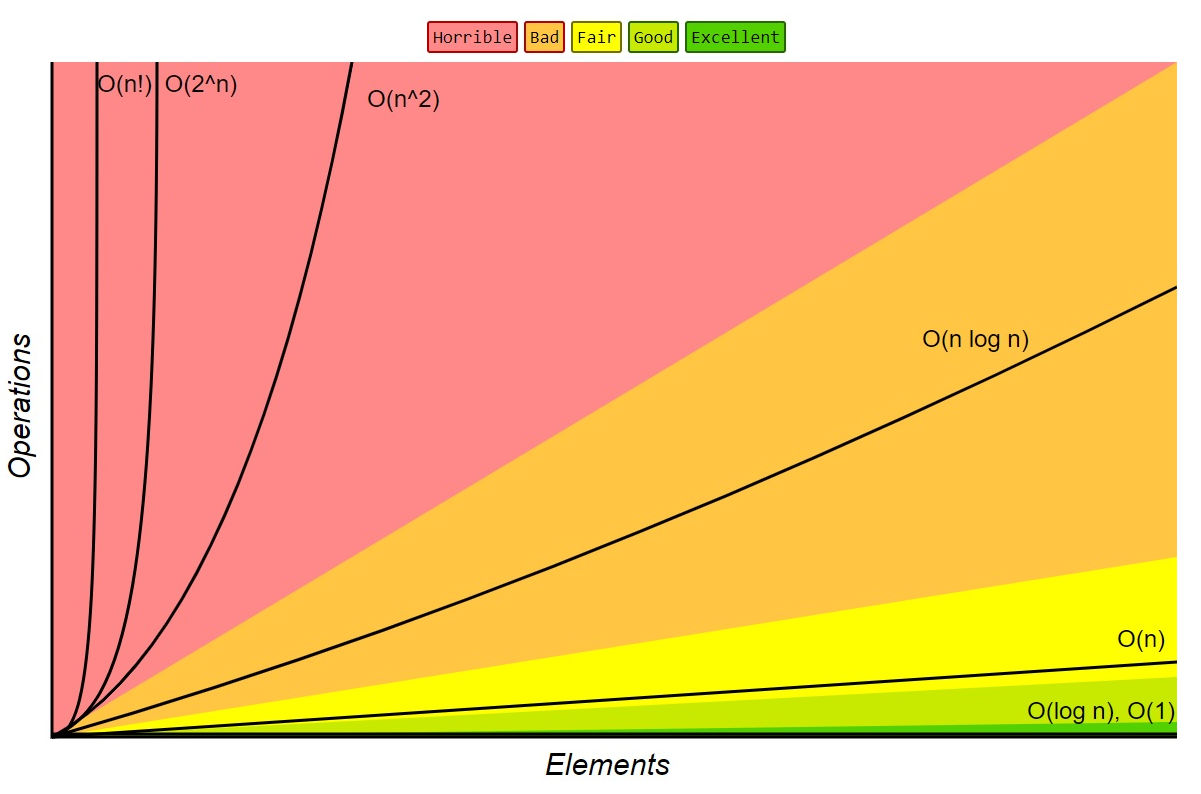
\includegraphics[scale=0.4]{bigO.jpg}
\end{frame}

\section[Insert]{Insertion Sort!}
\begin{frame}{Insertion Sort!}
Bubblesort works, but it contains redundant examinations!  
\begin{itemize}
\item Insertion Sort minimizes the number of examinations that do not lead to a swapping operation.
\item Insertion sort only makes one pass of the array, sorting as it goes.
\item The overall algorithm is to examine each element in the array, passing the element back through the sorted section of the array until the correct spot is found for it.  
\end{itemize}
\end{frame}

\begin{frame}{Insertion Sort Pass Back Procedure}
\begin{itemize}
\item For each element of the array:
\begin{itemize} 
\item The unsorted element is compared to the largest element in the sorted array, which will always be adjacent to it.  
\item If the unsorted element is smaller than the element it has been compared to, those two elements are swapped, and the unsorted element is then compared to the next largest element in the sorted section.
\item This proceeds until the unsorted element is greater than or equal to the element it has been compared to.  This means it has been sorted.  
\item At this point, the size of the section of the array we consider sorted increases by one, and we examine the next unsorted element.  
\end{itemize}
\end{itemize}
\end{frame}

\begin{frame}{Visualizing Insertion Sort}
\center
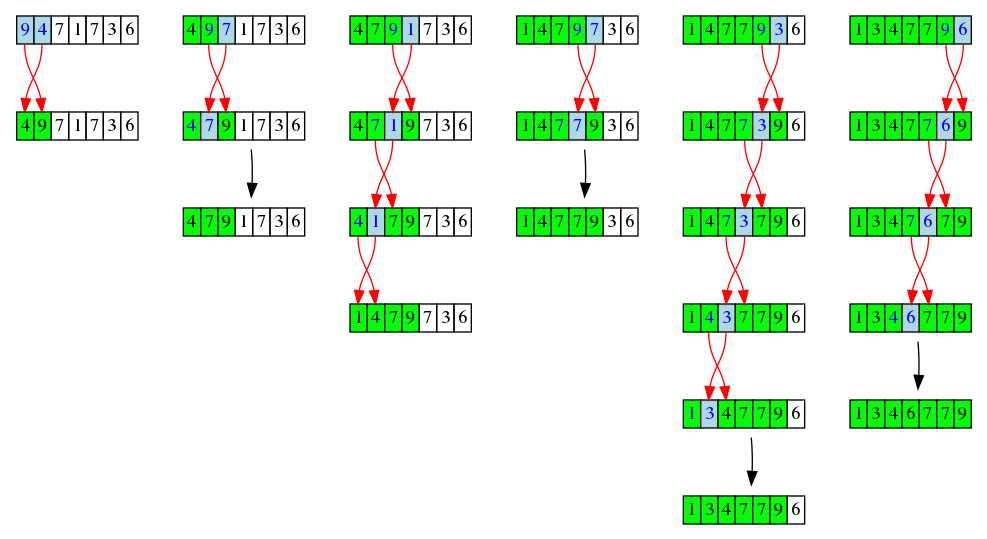
\includegraphics[scale=0.25]{graphs/insertionsort.png}
\end{frame}

\begin{frame}{Analysis of Insertion Sort}
\begin{itemize}
\item The number of swap operations we require for insertion sort is 13.   
\item The total number of examinations was 17, for an array of size 7.
\item With bubblesort, the operations it takes to sort each element \textbf{decreases} with the size of the sorted section.
\item With insertion sort, the operations it takes to sort each element \textbf{increases} with the size of the sorted section.  
\item Insertion sort is an \emph{adaptive} algorithm, since it's runtime is depended on the \textbf{sortedness} of the array
\begin{itemize}
\item Sortedness is a measure of how far off the array is from a sorted configuration. 
\item Sortedness is also sometimes called \textbf{degree of disorder}.  
\item The number of swaps performed in either bubblesort or insertion sort is a direct measure of sortedness.
\end{itemize}
\end{itemize}
\end{frame}

\begin{frame}{Best-Case / Worst Case Analysis}
\begin{itemize}
\item One candidate for the worst case scenario is an array in descending order: $\{9,7,7,6,4,3,1\}$
\begin{itemize}
\item For bubblesort, every examination would lead to a swap.  
\item Insertion sort would need the same number of swaps, so the worst-case runtime for insertion sort is $O(n^2)$, the same as bubblesort
\end{itemize}
\item The least disordered array (or best case scenario) is an array that has already been sorted: $\{1,3,4,6,7,7,9\}$
\begin{itemize}
\item For bubblesort, no examinations would lead to a swap.
\item Insertion sort only performs one operation per element (checking to see that it's correct.)
\item This means the number of operations performed is proportional to $n^1$, where $n$ is the length of the array.
\item The computational complexity is $O(n)$
\end{itemize}
\end{itemize}
\end{frame}

\section[Shell]{Shell Sort!}
\begin{frame}{Shellsort!}
Although insertion sort is an improvement over bubblesort, the number of swap operations that must be performed has not changed.  
\begin{itemize}
\item This is because each swap addresses one unit of disorder.  
\item It may be possible to increase our efficiency by performing swaps between array elements that are not adjacent! 
\item In \textbf{shellsort}, we extract a sub-array, sort it, and then put it back.
\item By selecting elements that are positionally distant, we can reduce large amounts of disorder quickly.
\item Shellsort is often used in embedded systems applications:
\begin{itemize}
\item The code to implement Shellsort is small, it is memory efficient, and does not use the call stack.
\end{itemize}
\end{itemize}
\end{frame}

\begin{frame}{Interleaving and H-gaps}
The key to shellsort is knowing how to break down the array into subarrays.  
\begin{itemize}
\item Sub arrays are formed by taking an element, skipping $h$ elements, then taking the next element, until the end of the array is reached.
\item The sequence of h-values used varies by implementation, with different sequences being proposed by different researchers (most recently in 2001).  
\begin{itemize}
\item The sequence is $(1, 4, 10, 23, 57, 132, 301, 701)$
\item This order was experimentally derived.  No equation has yet been discovered which can predict the next number in the sequence.  
\item The worst case performance of this sequence is currently unknown.  
\end{itemize}
\end{itemize}
\end{frame}

\begin{frame}{Visualizing H-Gaps 1}
\center
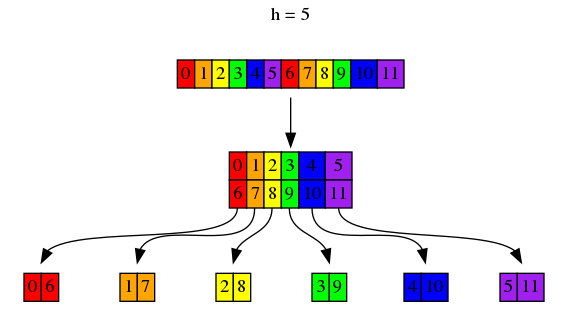
\includegraphics[scale=0.5]{graphs/shellsortSlicing.png}
\end{frame}

\begin{frame}{Visualizing H-Gaps 2}
\center
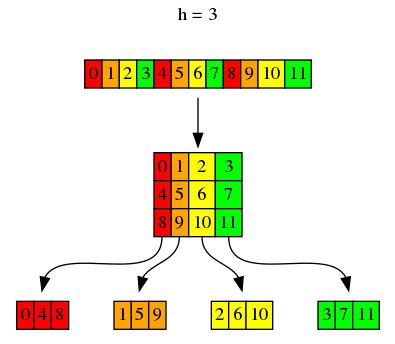
\includegraphics[scale=0.5]{graphs/shellsortSlicing2.png}
\end{frame}

\begin{frame}[fragile=singleslide]{Shellsort! (cont.)}
Once we have our sub-arrays established, we perform insertion sort on each one of them, and then put the elements back into the original array.
\begin{itemize}
\item Once all the sub arrays have been sorted and replaced for one h-value, we say that the array is \textbf{h-sorted}.  
\item The success of shellsort hinges on the fact that smaller h-sortings do not disorder larger ones. 
\begin{itemize}
\item E.g., if an array is 40-sorted, and we 14-sort it, the finished array is still 40-sorted.  
\end{itemize}
\item As long as the last h-value is 0 (which is just insertion sort), the array is guaranteed to be sorted!
\end{itemize}
\end{frame}

\begin{frame}{Visualizing Shellsort}
\center
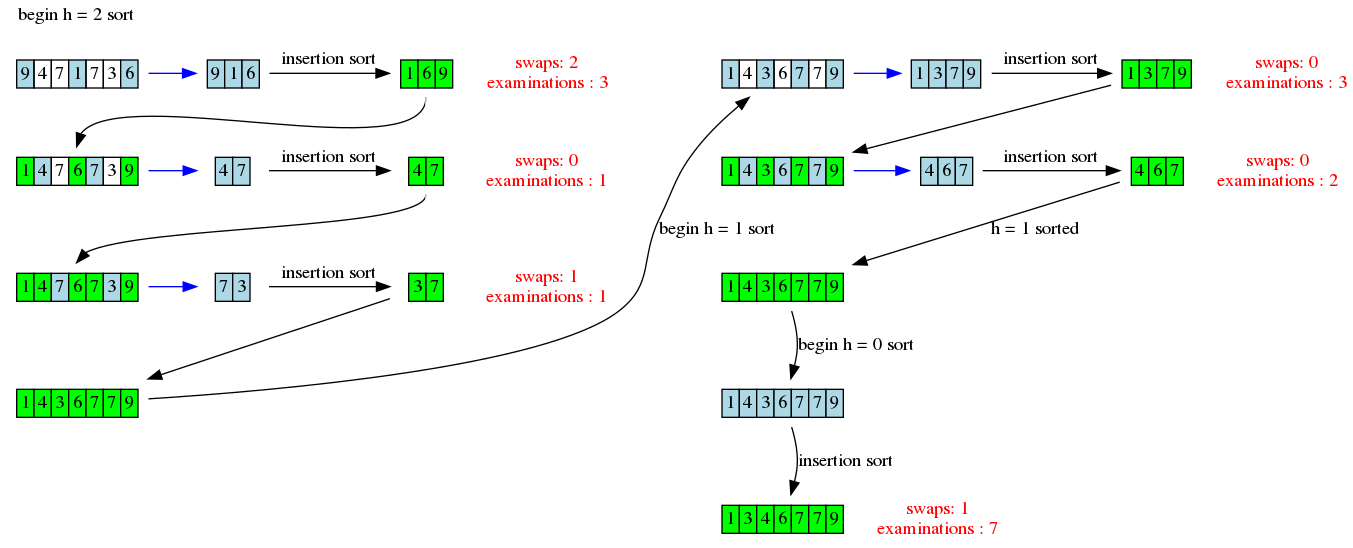
\includegraphics[scale=0.25]{graphs/shellsort.png}
\end{frame}

\begin{frame}{Analysing Shellsort}
\begin{itemize}
\item Total Swaps : 4(!!) 
\item Total Examinations : 17(!)
\item While the previous slide implies the sub-arrays are instantiated separatedly from original array, this does not need to be the case.  Shellsort may be performed without allocating new memory beyond the swap space insertion sort uses.  
\item The worst-case analysis for shellsort is highly dependent on the h-gap sequence. 
\begin{itemize}
\item Early versions (1960s) are guaranteed to be no worse than $O(n^{3/2})$
\item The best version we have results for are guaranteed to be no worse than $O(n^{4/3})$
\end{itemize}
\end{itemize}
\end{frame}

\section[Search]{Search Algorithms}
\begin{frame}{What is a Search Algorithm?}
In order to talk about search algorithms, we should first define them.  
\begin{itemize}
\item Given a data structure composed of elements and an element to search for, a \textbf{search algorithm} tests for the presence of the searched-for element in the data structure.
\item The output can be either a True/False value, or the index of the searched-for element.
\item Search algorithms may be applied to many diverse types of data structures, but we're going to focus on arrays for now.
\end{itemize}
\end{frame}

\begin{frame}{Linear Search}
The most straightforward approach is \textbf{Linear Search}
\begin{itemize}
\item Beginning at the first element of the array, each element is compared to the searched for element.  
\item The algorithm returns \texttt{True} as soon as the item appears.
\item If the end of the array is reached before the item is found, return \texttt{False}
\begin{itemize}
\item Worst case complexity is $O(n)$ (item isn't present)
\item The average position of the sought for element is the middle, assuming uniform randomness, thus $O(n/2)$
\begin{itemize}
\item Though this is still $O(n)$, because we only care about the power, not the constant.  
\end{itemize}
\end{itemize}
\end{itemize}
\end{frame}

\begin{frame}{Binary Search}
We have to use Linear search if we can't assume anything about the data.
\begin{itemize}
\item In algorithm design, if data has \emph{known properties}, we can use this information to come up with better algorithms.
\item If the array is already sorted, we can use \textbf{Binary Search}, an algorithm that has a worst-case complexity of $O(log_2(n))$! 
\item Rather than looking at each item, binary search narrows the field of search iteratively, until the value is found (or not).
\end{itemize}
\end{frame}

\begin{frame}{Binary Search Procedure}
Let's say we are looking for $x$ in $A$:
\begin{enumerate}
\item Create two variables to keep track of the search range:
\begin{itemize}
\item $a$ to track the lower bound
\item $b$ to track the upper bound
\end{itemize}
\item Examine the number at index $m = \lfloor \frac{a+b}{2} \rfloor$
\begin{enumerate}
\item If the numbers at $m$, $a$, or $b$ equal to $x$, we have found $x$! 
\item If this number is less than $x$, we know that $x$ must be at a higher index than  $\lfloor \frac{a+b}{2} \rfloor$.
\begin{itemize}
\item Set $a$ to $\lfloor \frac{a+b}{2} \rfloor$ and return to step 2.
\end{itemize}
\item If this number is greather than $x$, we know that $x$ must be at a lower index than  $\lfloor \frac{a+b}{2} \rfloor + 1$.
\begin{itemize}
\item Set $b$ to $\lfloor \frac{a+b}{2} \rfloor - 1$ and return to step 2.
\end{itemize}
\end{enumerate}
\end{enumerate}
\end{frame}

\begin{frame}{Visualizing Binary Search}
\center
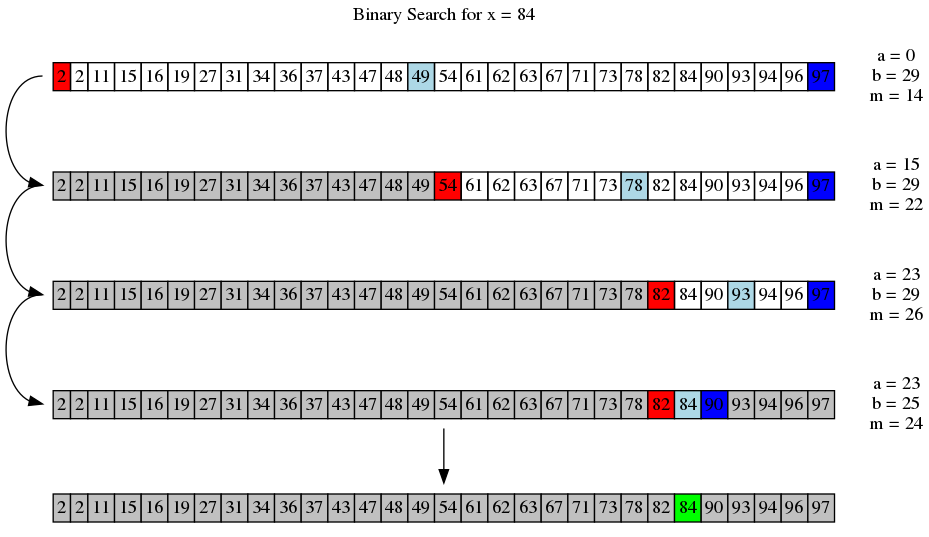
\includegraphics[scale=0.3]{graphs/binSearch.png}
\end{frame}

\begin{frame}{Analysing Binary Search}
\begin{itemize}
\item Because we are halving the search space with each step, this is a $O(log_2(n))$ algorithm 
\begin{itemize}
\item This is considered a ``good'' complexity.
\item Sometimes, $log_2()$ is written as $lg()$
\item Sometimes, $log_2()$ is written as $log()$
\begin{itemize}
\item This is sometimes because we're ignoring the base of the logarithm for Big O reasons
\item This is sometimes because when a computer scientist says ``logarithmic'', the base 2 is implied because it's computer science.
\end{itemize}
\end{itemize}
\item This means that we can deal with 1000 items in only 10 steps, and we can deal with 1000000 items in only 20! 
\item This is the \emph{worst case runtime!}
\end{itemize}
\end{frame}

\begin{frame}{The Last Slide Comic}
The Travelling Salesman Problem...
\center
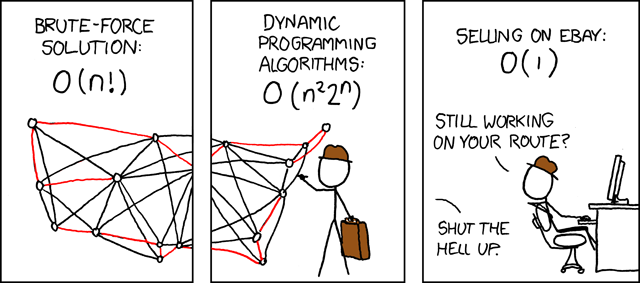
\includegraphics[scale=0.4]{travelling_salesman_problem.png}
\end{frame}

\end{document}
